\chapter{CÁC QUY ĐỊNH CHUNG}
\label{chap:quydinh}
\pagenumbering{arabic}



\section{Giới thiệu chung}
\label{sec:gtchung}
	\quad Đồ án/khóa luận tốt nghiệp (sau đây gọi tắt là ĐATN) được qui định về qui cách trình bày, sinh viên cần đảm bảo đúng qui cách này trước khi in và nộp quyển. Cấu trúc chung của đồ án khi đóng quyển gồm các phần thứ tự như sau:
\begin{enumerate}
	\item Bìa trước của ĐATN: mục chuyên ngành có thể ghi hoặc không ghi; với khóa luận tốt nghiệp sẽ thay chữ ``Đồ án tốt nghiệp'' thành ``Khóa luận tốt nghiệp''
	\item Đề tài tốt nghiệp (phải có chữ ký của giáo viên hướng dẫn)
	\item Phần ``Lời cảm ơn'' và ``Tóm tắt đồ án'' (trình bày trong 1 trang và sinh viên cần ký tên, ghi rõ họ tên tại trang này)
	\item Mục lục
	\item Danh mục hình vẽ
	\item Danh mục bảng biểu
	\item Các chương thuộc nội dung đồ án
	\item Phụ lục(nếu có)
 	\item Tài liệu tham khảo
	\item Bìa cuối đồ án
\end{enumerate}
Đây là bản hướng dẫn đồng thời cũng là mẫu sử dụng khi viết đồ án. Người dùng có thể copy và dán nội dung cần thiết vào các mục trong mẫu này để giữ được định dạng (format) của văn bản.



\section{Sử dụng các định dạng văn bản theo quy định}
\label{sec:dinhdang}

	\subsection{Qui định về căn lề văn bản}
	\label{ssec:canle}
Nội dung phần chữ căn đều 2 bên (mặc định trong \LaTeX{} rồi)	
	
Căn lề phía trên, dưới, trái, phải của văn bản như sau:\\
%\usepackage[left=3.5cm,right=2.5cm,top=2cm,bottom=2cm]{geometry}
khoảng cách giữa các đoạn văn bản:

\begin{figure}[h]
\centering
	\caption{Thức yêu Hoài}
	
\includegraphics[scale=0.1]{figures/thuchoai}
	\label{fig:th}
	
\end{figure}
\begin{verbatim}
\setlength{\parskip}{2cm}
 khoảng cách giữa các dòng: \usepackage{setspace}
 \setstretch{1.6} %%  \doublespacing
 
Def AppendAndSort(Node)
	if head == None
	\	Node = head
		Node = tail
 	if Node.data >= head.data
	Node.next = head
	head = Node
 	else
		if Node.data <= tail.data
			tail.next = Node
			tail = Node
		if Node.data > tail.data
			cur = head
 			while cur.data != tail
				if Node.data < cur.data and Node.data > cur.next.data
					Node.next = cur.next
					cur.next = Node
					cur = cur.next

\end{verbatim}


từ muốn chú thích\footnote{nội dung chú thích}
…<từ muốn chú thích>\footnote{nội dung chú thích}
	\subsection{Tạo lề cho văn bản in 2 mặt}
	\label{ssec:taole}
	
\begin{verbatim}
#include <stdio.h>
int main()
{
    printf{"The chemistry website of vietnam\n"};
    return 1;
}
\end{verbatim}
	
	\subsection{Tạo chương mơi}
	\label{ssec:taochuong}
	
	\subsection{Tạo tiêu đề các cấp}
	\label{ssec:taotieude}
	
	\subsection{Hình vẽ - Đồ thị}
	\label{ssec:hd}
Hình vẽ hoặc đồ thị (gọi tắt là hình vẽ) có hiệu quả cao khi sử dụng để minh họa cho các nội dung cần tóm lược, do vậy nên được sử dụng để tránh việc đưa các thông tin quá dài.
Hình vẽ có kích thước chiều rộng không quá 75\% của chiều rộng nội dung phần chữ, căn lề giữa (trừ các trường hợp đặc biệt có thể rộng hơn hoặc sử dụng trang ngang kiểu Landscapse ).
	

	\subsection{Bảng biểu}
	\label{ssec:bang}
Tương tự như hình vẽ, bảng biểu nên có chiều rộng không quá 75\% chiều rộng phần chữ của nội dung. Tiêu đề bảng biểu đặt phía trên bảng với cách tạo định dạng tương tự. Bảng biểu nên bố trí để nằm trọn vẹn trong một trang, tránh việc cùng một bảng bị ngắt sang trang khác.	
	
	\subsection{Phương trình}
	\label{ssec:pt}
Tôi yêu toán: $x^n + x^n \neq z^n \forall n \neq 2$ là định lý Fermat lớn.\newline

Định lý Fermat lớn:
\begin{equation}
x^n + x^n \neq z^n \quad\forall n \neq 2
\label{eq:fermat}
\end{equation}
Bạn có thể chứng minh bất đẳng thức (\ref{eq:fermat})?
	
	
\section{Tạo tham chiếu chéo giữa các đoạn văn bản}
\label{sec:thamchieucheo}

\section{Tạo danh mục tài liệu tham khảo}
\label{sec:taodanhmuc}

\section{Cập nhật lại các ghi chú và tham chiếu}
\label{sec:capnhat}

\section{Tạo danh mục hình vẽ}
\label{sec:hinhve}

\section{Tạo danh mục bảng biểu}
\label{sec:bangbieu}

\section{Chú thích cuối trang}
\label{sec:chuthich}
\renewcommand{\thefootnote}{**}
từ muốn chú thích\footnote{nội dung chú thích}

\section{Qui cách đóng quyển}
\label{sec:dongquyen}
	\quad Phần bìa trước chế bản theo qui định; bìa trước và bìa sau là giấy liền khổ. Sử dụng keo nhiệt để dán gáy khi đóng quyển thay vì sử dụng băng dính và dập ghim.\newline
	\begin{figure}[h]
	\centering
		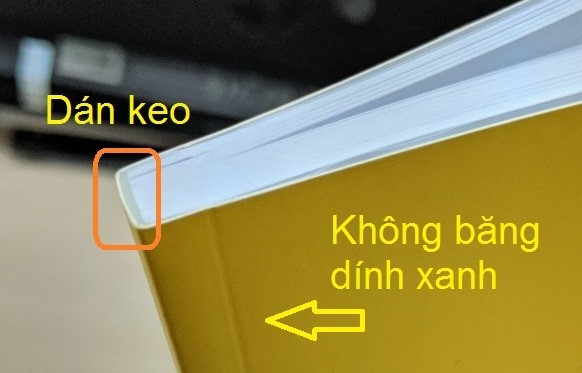
\includegraphics[scale=1]{figures/fig1}
		\caption{Dán keo}
		
		
\includegraphics[scale=0.3]{figures/fig2}
		\caption{Không băng dính xanh}
	\end{figure}
	
Phần gáy ĐATN cần ghi các thông tin tóm tắt sau:
Kỳ~làm~ĐATN~-~Ngành~đào~tạo~-~Họ~và~tên~sinh~viên~-~Mã~số~sinh~viên.
\vspace{2cm}

Ví dụ:

\textbf{2019.1 - VẬT LÝ KỸ THUẬT - NGUYỄN VĂN A - 20141234}

Qui cách ghi chữ phần gáy như hình sau:

\begin{figure}
\centering
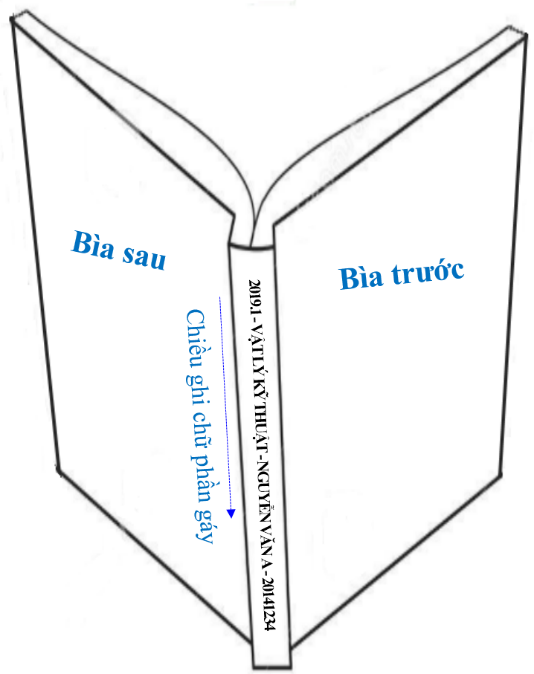
\includegraphics[scale=0.7]{figures/fig3}
\caption{Ghi chữ phần gáy}
\end{figure}

